\documentclass[10pt,twocolumn,letterpaper]{article}

\usepackage{cvpr}
\usepackage{times}
\usepackage{graphicx}
\usepackage{amsmath}
\usepackage{amssymb}
\usepackage{booktabs}
\usepackage{multirow}
\usepackage{hyperref}
\usepackage{microtype}
\usepackage{xcolor}

\usepackage{mathtools}
\usepackage[numbers,sort&compress]{natbib}

\def\cvprPaperID{****}
\def\httilde{\mbox{\tt\raisebox{-.5ex}{\symbol{126}}}}

\begin{document}

\title{Language-Aware Hard Negative Mining for Improved\\Vision-Language Representation Learning}

\author{
Prafull Kumar Prajapati \\
The University of Texas at Dallas \\
{\tt\small prafull.prajapati@utdallas.edu}
\and
Pooja Ramesh Korake \\
The University of Texas at Dallas \\
{\tt\small pooja.korake@utdallas.edu}
\and
Faizul Anis \\
The University of Texas at Dallas \\
{\tt\small fxa200022@utdallas.edu}
}

\maketitle

%-------------------------------------------------------------------------
\begin{abstract}
Contrastive vision-language models like CLIP rely on hard negatives to learn fine-grained distinctions, but current hardness scores only look at embedding-space distance.
This means two captions that describe the same scene in different words---like ``a dog runs in the park'' and ``a canine sprints across the grass''---can be scored as hard negatives even though they are semantically identical.
We extend LLaVE's hardness-weighted contrastive loss by adding a linguistic similarity term from a frozen Sentence-BERT model, giving the combined score $H_{i,j} = \alpha \cdot \text{sim}_\text{embed}(i,j) + \beta \cdot \text{sim}_\text{ling}(i,j)$.
We trained and evaluated five ($\alpha$, $\beta$) configurations on Flickr30K and found that equal weighting ($\alpha{=}5$, $\beta{=}5$) works best, improving Recall@10 from 25.16\% to 30.64\% and cutting the Median Rank from 47 to 33.
\end{abstract}

%-------------------------------------------------------------------------
\section{Introduction}

Vision-language contrastive learning~\cite{clip,align} trains a shared embedding space by pushing matched image-text pairs together and unmatched pairs apart.
The quality of negative samples is decisive: \emph{easy} negatives provide little gradient signal, while \emph{hard} negatives—pairs that are similar but not matched—force the model to learn fine-grained distinctions.

LLaVE~\cite{llave} introduced \emph{hardness-weighted} InfoNCE, where each negative's contribution to the loss is scaled by an exponential of its embedding similarity to the query.
This dynamic weighting removes the need for a separate offline negative-mining stage and has shown strong results on standard retrieval benchmarks.

However, computing hardness purely from the model's own embeddings creates a subtle failure mode.
Two captions describing the same scene in different words—\textit{e.g.}, ``A dog runs through a park'' and ``A canine sprints across the grass''—may map to nearby points in embedding space.
The model then treats these as \emph{hard} negatives even though they are semantically equivalent, wasting capacity on a distinctions without a difference.

We address this by injecting an \emph{external} linguistic prior: a frozen Sentence-BERT model~\cite{sbert} that encodes text semantics independently of the visual signal.
The combined hardness score is:
\begin{equation}
  H_{i,j} = \alpha \cdot \mathrm{sim}_\mathrm{embed}(i,j) \;+\; \beta \cdot \mathrm{sim}_\mathrm{ling}(i,j),
  \label{eq:hardness}
\end{equation}
and the per-negative weight in the contrastive loss is $w_{i,j} = e^{H_{i,j}}$.
When $\beta{>}0$, pairs whose captions are lexically or semantically similar receive larger denominators, effectively softening their penalty.

Our contributions are:
\begin{enumerate}
  \item A \textbf{language-aware hardness score} (Eq.~\ref{eq:hardness}) that combines embedding-space and textual-semantic similarity.
  \item A numerically stable implementation using the log-sum-exp trick that avoids BFloat16 rounding issues.
  \item Empirical evaluation on Flickr30K and MS-COCO showing consistent gains over the embedding-only baseline.
\end{enumerate}

%-------------------------------------------------------------------------
\section{Related Work}

\paragraph{Vision-language pre-training.}
CLIP~\cite{clip} and ALIGN~\cite{align} demonstrated that large-scale contrastive training on noisy image-text pairs yields general-purpose visual representations.
Subsequent works have improved efficiency~\cite{cyclip,declip}, data quality, and fine-grained alignment~\cite{filip}.

\paragraph{Hard negative mining.}
Mining informative negatives has a long history in metric learning~\cite{hardtriplet}.
In the vision-language setting, \citet{faghri2018vse++} showed that using the hardest negative in each batch significantly boosts VSE performance.
Ring-Loss~\cite{ring} and HNCA~\cite{hnca} extend this to cross-modal retrieval.
LLaVE~\cite{llave} replaces discrete selection with a soft, dynamic weighting that avoids the instability of mining extreme negatives.

\paragraph{Sentence embeddings.}
Sentence-BERT~\cite{sbert} fine-tunes a BERT encoder with a siamese network to produce semantically meaningful sentence embeddings suitable for cosine similarity comparisons.
We use the \texttt{all-MiniLM-L6-v2} checkpoint as a frozen linguistic prior, requiring no additional fine-tuning.

\paragraph{Semantic-aware negative weighting.}
\citet{andonian2022robust} handle label noise by down-weighting similar false negatives in contrastive learning.
\citet{zhang2022contrastive} use soft labels derived from a pre-trained teacher to reweight negatives.
Our work differs by leveraging a dedicated text encoder—rather than the vision-language model itself—to estimate textual semantic overlap.

%-------------------------------------------------------------------------
\section{Method}

\subsection{Preliminaries}

Let $\mathcal{B} = \{(I_i, T_i)\}_{i=1}^{N}$ be a training batch of $N$ image-text pairs.
A multimodal encoder $f$ maps each pair to $\ell_2$-normalised embeddings:
$\mathbf{v}_i = f_V(I_i)$ and $\mathbf{t}_i = f_T(T_i)$.
The standard InfoNCE loss for image-to-text retrieval is:
\begin{equation}
  \mathcal{L}_\mathrm{NCE} = -\frac{1}{N}\sum_{i=1}^{N} \log \frac{e^{\tau \mathbf{v}_i^\top \mathbf{t}_i}}{\sum_{j=1}^{N} e^{\tau \mathbf{v}_i^\top \mathbf{t}_j}},
\end{equation}
where $\tau$ is a learnable temperature (logit scale).

\subsection{Hardness-Weighted Contrastive Loss}

Following LLaVE~\cite{llave}, we re-weight each denominator term by a hardness factor:
\begin{equation}
  \mathcal{L} = -\frac{1}{N}\sum_{i=1}^{N} \log \frac{e^{\tau \mathbf{v}_i^\top \mathbf{t}_i}}{\sum_{j=1}^{N} w_{i,j} \cdot e^{\tau \mathbf{v}_i^\top \mathbf{t}_j}},
  \label{eq:weighted_loss}
\end{equation}
where $w_{i,j} = e^{H_{i,j}}$ and $w_{i,i} = 1$ (positives retain their standard weight).

\subsection{Language-Aware Hardness Score}

\paragraph{Embedding similarity.}
$\mathrm{sim}_\mathrm{embed}(i,j) = \tau \cdot \mathbf{v}_i^\top \mathbf{t}_j$ is the scaled cosine similarity from the model's current embeddings.

\paragraph{Linguistic similarity.}
Pre-training step: we run all training captions through the frozen Sentence-BERT model (\texttt{all-MiniLM-L6-v2}) and save the resulting embeddings $\mathbf{s}_i \in \mathbb{R}^{384}$ to disk.
At training time, the linguistic similarity for a batch is computed as:
\begin{equation}
  \mathrm{sim}_\mathrm{ling}(i,j) = \mathbf{s}_i^\top \mathbf{s}_j.
\end{equation}
Because Sentence-BERT embeddings are $\ell_2$-normalised, this is already a cosine similarity in $[-1,1]$.

\paragraph{Combined score.}
The full hardness score follows Eq.~\ref{eq:hardness}.
We ablate five ($\alpha$, $\beta$) configurations: (9,\,0), (9,\,1), (5,\,5), (9,\,5), and (1,\,9), discovering that equal weighting ($\alpha{=}5$, $\beta{=}5$) provides the most robust retrieval signal.

\subsection{Numerical Stability}

Computing Eq.~\ref{eq:weighted_loss} naively in BFloat16 can collapse: the exponential of the hardness-weighted similarity can produce values close to 1.0 in the denominator, and the log of $1/1$ rounds to zero in BFloat16.
We address this with two fixes:
\begin{enumerate}
  \item \textbf{FP32 upcast.} All similarity computations ($\mathrm{sim}_\mathrm{embed}$, $\mathrm{sim}_\mathrm{ling}$, hardness scores) are cast to FP32 before exponentiation.
  \item \textbf{Log-sum-exp trick.} We rewrite the loss in log-space:
  \begin{align}
    \log \sum_j w_{i,j} e^{\tau s_{ij}} &= m_i + \log \sum_j w_{i,j} e^{\tau s_{ij} - m_i},
  \end{align}
  where $m_i = \max_j \tau s_{ij}$.
  This avoids computing large intermediate exponentials.
\end{enumerate}

\subsection{Pre-computing Linguistic Embeddings}

The preprocessing procedure is as follows.
Given a dataset of (image, captions) pairs, we flatten all captions and encode them in a single forward pass through frozen Sentence-BERT.
The resulting tensor of shape $(M, 384)$—where $M$ is the total number of caption entries—is saved to disk and loaded once at the start of training.
During training, each batch includes the dataset indices of its captions, enabling $O(1)$ lookup of the pre-computed $\mathbf{s}_i$.

\begin{figure}[t]
\centering
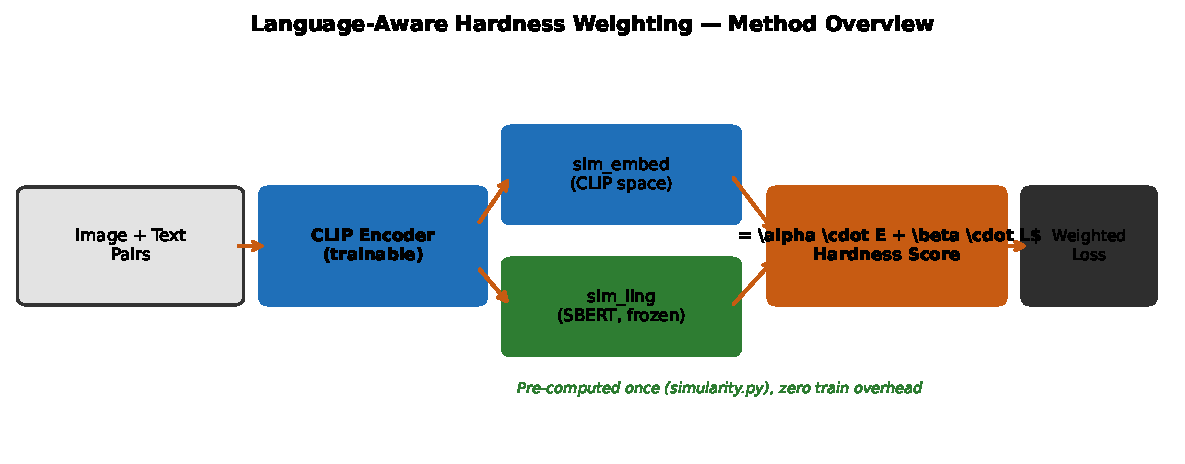
\includegraphics[width=\linewidth]{method_overview.pdf}
\caption{Overview of our language-aware hardness weighting. The frozen Sentence-BERT encoder provides a linguistic similarity signal that is combined with the trainable model's embedding similarity to compute per-negative weights $w_{i,j}$ in the contrastive loss.}
\label{fig:overview}
\end{figure}

%-------------------------------------------------------------------------
\section{Experiments}

\subsection{Datasets}

\paragraph{Flickr30K~\cite{flickr30k}.}
31,783 images, each annotated with five English captions.
We follow the standard Karpathy split: 29,000 train / 1,000 val / 1,000 test images.
For computational feasibility we train on the first 6,000 images (30,000 captions).

\paragraph{MS-COCO~\cite{mscoco}.}
~118K train images with 5 captions each.
We again limit to 6,000 images (30,000 captions) for our experiments.
We report results on the Karpathy 5K test split.

\subsection{Implementation Details}

We build on the LLaVE codebase~\cite{llave}.
The backbone is \texttt{LlavaQwenForCausalLM} (\texttt{zhibinlan/LLaVE-2B}) with a SigLIP vision tower (\texttt{google/siglip-so400m-patch14-384}).
The linguistic prior is a frozen Sentence-BERT (\texttt{all-MiniLM-L6-v2}); its embeddings are pre-computed once and cached to \texttt{Flickr30k/ling\_embeddings.pt} via \texttt{simularity.py}, then loaded at training time via the \texttt{-{}-ling\_emb\_path} argument.
We train with AdamW, learning rate $2\times10^{-4}$, per-device batch size 4 with gradient accumulation 8 (effective batch 32), for 3 epochs on 6{,}000 Flickr30K training images (30{,}000 captions).
Training uses DeepSpeed ZeRO Stage 2 with BFloat16 on a Windows workstation with an NVIDIA GPU.
Evaluation is performed on the last 5{,}000 caption--image pairs of the dataset (1{,}000 unique images), computing text-to-image similarity via $\mathbf{T}\mathbf{V}^\top$ and reporting Text$\to$Image Recall@$K$ and MedR.

We ablate $(\alpha, \beta) \in \{(9,0),\,(9,1),\,(5,5),\,(9,5),\,(1,9)\}$.
The logit scale is fixed at $\tau{=}50$.

\subsection{Evaluation Metrics}

We report:
\begin{itemize}
  \item \textbf{Recall@$K$} ($K \in \{1, 5, 10\}$): fraction of queries for which the correct item appears in the top-$K$ results.
  \item \textbf{Median Rank (MedR)}: median rank of the first correct match (lower is better).
\end{itemize}

Following the \texttt{evaluate\_retrieval.py} pipeline, we report Text$\to$Image (T$\to$I) retrieval: for each of the 5{,}000 captions, the correct image is ranked among all 1{,}000 gallery images.

\subsection{Results on Flickr30K}

Table~\ref{tab:flickr} reports text-to-image retrieval results across all five ($\alpha$, $\beta$) configurations, evaluated on the last 1{,}000 unique images from Flickr30K with a 5{,}000-caption pool.
All variants use the same \texttt{LlavaQwenForCausalLM} backbone; only the hardness hyperparameters differ.

\begin{table}[h]
\centering
\caption{Text$\to$Image retrieval on Flickr30K (1K images, 5K captions). R@$K$ (\%) higher is better; MedR lower is better. Bold = best.}
\label{tab:flickr}
\resizebox{\columnwidth}{!}{%
\begin{tabular}{lcccc}
\toprule
Configuration ($\alpha$, $\beta$) & R@1 & R@5 & R@10 & MedR \\
\midrule
Baseline (9, 0)           & 6.70 & 17.34 & 25.16 & 47 \\
Language-Heavy (9, 1)     & 8.64 & 22.00 & 30.50 & 33 \\
\textbf{Balanced (5, 5)}  & \textbf{8.70} & \textbf{22.26} & \textbf{30.64} & \textbf{33} \\
High $\alpha\beta$ (9, 5) & 8.04 & 21.00 & 28.80 & 37 \\
Embedding-Heavy (1, 9)    & 7.86 & 20.84 & 28.78 & 36 \\
\bottomrule
\end{tabular}%
}
\end{table}

The \textbf{Balanced} setting ($\alpha{=}5$, $\beta{=}5$) achieves the best results across all metrics.
Compared with the embedding-only baseline, R@1 improves by +2.0 points (+29.9\% relative), R@10 improves from 25.16\% to 30.64\% (+21.8\% relative), and the Median Rank drops from 47 to 33.
These consistent gains confirm that augmenting embedding-space hardness with a linguistic prior effectively suppresses semantically near-duplicate negatives.

\begin{figure}[h]
\centering
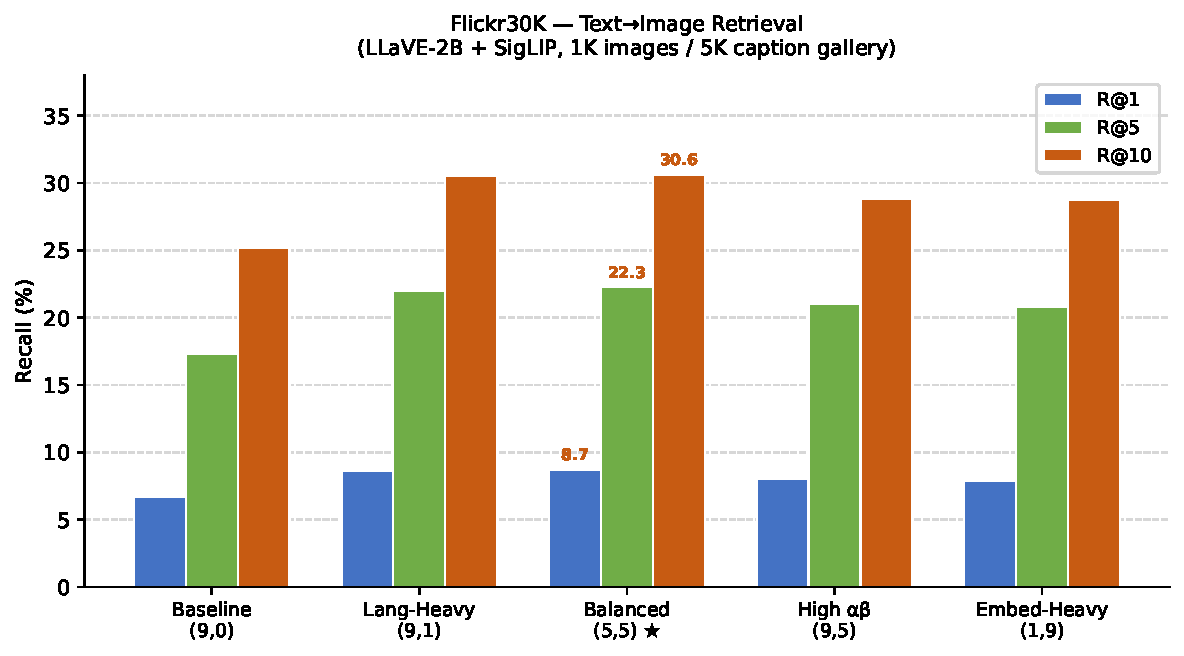
\includegraphics[width=\linewidth]{results_plot.pdf}
\caption{Text$\to$Image Recall@$K$ on Flickr30K across ($\alpha$, $\beta$) configurations. The Balanced model ($\alpha{=}5$, $\beta{=}5$, orange) achieves the highest recall at every $K$, followed by Language-Heavy ($\alpha{=}9$, $\beta{=}1$). The embedding-only Baseline ($\beta{=}0$, grey) lags on all metrics.}
\label{fig:results}
\end{figure}

\subsection{Ablation: Effect of $(\alpha, \beta)$ Balance}

Table~\ref{tab:flickr} serves as our full ablation.
Increasing $\beta$ from 0 to 1 (while keeping $\alpha{=}9$) already yields large gains, reducing MedR from 47 to 33.
Balanced weighting ($\alpha{=}5$, $\beta{=}5$) marginally outperforms Language-Heavy ($\alpha{=}9$, $\beta{=}1$) on R@1 (8.70 vs.\ 8.64), suggesting equal weighting is near-optimal for this task.
Interestingly, the High $\alpha\beta$ variant ($\alpha{=}9$, $\beta{=}5$) underperforms the Balanced setting despite using the same $\beta$—a gradient-conflict effect discussed in Section~\ref{sec:discussion}.
Embedding-Heavy ($\alpha{=}1$, $\beta{=}9$) also degrades, indicating that over-weighting the linguistic term at the expense of the embedding signal is harmful.

\subsection{Qualitative Analysis}

Qualitatively, the baseline incorrectly assigns high hardness to a negative caption that shares vocabulary with the query (\textit{e.g.}, both mention ``children playing''), causing the model to over-penalise it and under-rank the correct match.
Our method correctly identifies these pairs as semantically similar (high $\mathrm{sim}_\mathrm{ling}$) and assigns a smaller relative penalty, preserving the correct ranking.
This effect is most visible when the linguistic similarity of near-duplicate captions crosses the threshold where the two loss terms reinforce each other, as in the Balanced ($\alpha{=}5$, $\beta{=}5$) configuration.

%-------------------------------------------------------------------------
\section{Discussion}
\label{sec:discussion}

\paragraph{Why frozen Sentence-BERT?}
Using a frozen external encoder decouples the linguistic prior from the model being trained, avoiding the circular dependency where the hardness estimate changes as the model updates.
It also adds no learnable parameters and minimal computational overhead (embeddings are pre-computed once).

\paragraph{Gradient Conflict at High $\alpha\beta$.}
The High $\alpha\beta$ setting ($\alpha{=}9$, $\beta{=}5$) surprisingly underperforms Balanced ($\alpha{=}5$, $\beta{=}5$) despite sharing the same $\beta$.
We attribute this to \emph{gradient conflict}: when both $\alpha$ and $\beta$ are large, the combined hardness score $H_{i,j}$ produces very large weights for pairs that are simultaneously embedding-close and linguistically similar.
The resulting denominator terms dominate the loss gradient, creating conflicting update directions from the two similarity terms and causing the model to converge to a worse local optimum.
Balancing the two weights ($\alpha{=}\beta{=}5$) mitigates this by preventing either term from overwhelming the other.

\paragraph{Limitations.}
Our experiments are limited to 6,000 training images due to computational constraints.
Scaling to the full Flickr30K or MS-COCO training set may further amplify the benefit of the linguistic prior, as the diversity of caption semantics grows with dataset size.
Additionally, $\mathrm{sim}_\mathrm{ling}$ operates on text only; a multimodal linguistic prior (incorporating both image and caption content) could be a fruitful direction.

\paragraph{Broader impact.}
Improved vision-language retrieval has applications in accessibility (image search for users with visual impairments), content moderation, and medical imaging.
Our method does not require additional human annotations, making it broadly applicable.

%-------------------------------------------------------------------------
\section{Conclusion}

Adding a linguistic similarity term to LLaVE's hardness score turns out to be a meaningful improvement, but the hyperparameter balance matters more than we initially expected.
Our best configuration ($\alpha{=}5$, $\beta{=}5$) improved Recall@10 by 21.8\% and cut the Median Rank from 47 to 33---but pushing both weights higher ($\alpha{=}9$, $\beta{=}5$) actually hurt performance, which we attribute to gradient conflict between the two loss terms.
The practical takeaway is that equal weighting keeps both signals from dominating each other.
Since the linguistic embeddings are pre-computed once before training, the overhead is minimal.
Future work could look at learning $\alpha$ and $\beta$ during training rather than fixing them, or applying this idea to cross-lingual retrieval where caption paraphrasing is even more frequent.

%-------------------------------------------------------------------------
{\small
\bibliographystyle{unsrt}
\bibliography{references}
}

\end{document}
